\chapter{Grundlagen}
\label{chap:basics}
\todo[size=\small, inline]{Evtl. besseren Namen für Kapitel "`Grundlagen"' finden $\rightarrow$ Grundlegende Algorithmen/Techniken?!}%
\textbf{Hier kommt nur rein was ICH mache!}\\
An dieser Stelle soll zunächst ein Überblick über die in der vorliegenden Arbeit verwendeten Techniken gegeben werden. Diese beinhalten unter anderem Algorithmen der Computergrafik, welche Datenstrukturen benutzt werden und wie die Speicherverwaltung angesprochen wird.

\section{Datenstrukturen}
\label{sec:basics:datenstrukturen}
\textbf{Wofür und warum?!}\\
3D-Modelle aus Computer Aided Design - Anwendungen (CAD) werden üblicherweise nach ihrer Funktion gruppiert. Das mag beim Entwurf solcher Systeme auch praktisch sein, beim ihrer Visualisierung kann dies jedoch zu Problemen führen. Bei CAD-Modellen in Größenordnung der Boeing 777\footnote{\todo[size=\small, inline]{Boeing Herkunftshinweis verschieben an die erste Stelle wo es erwähnt wird.}%
Das 3D-Modell der Boeing 777 wurde freundlicherweise zur Verfügung gestellt von The Boeing Company, Seattle, WA, USA.} (ca. 350 Millionen Dreiecke) ist es wichtig, dass diese in eine geeignete räumliche Unterteilung überführt werden. Da ein Out-Of-Core-Renderer entwickelt wurde, findet ein ständiges Laden und Verwerfen von Teilmodellen statt. Je länger ein Renderer benötigt um herauszufinden, welche Teile des Modells er verwerfen kann und welche er als erstes anfordern sollte, desto länger braucht er auch um ein Bild zu erstellen. In dieser Arbeit wurde als hierarchische räumliche Unterteilung ein Randomized Sampletree (\ref{sec:basics:sampletree}) und zum Vergleich ein Loose Octree gewählt.

\subsection{Loose Octree}
\label{sec:basics:octree}
\textbf{Warum ein Loose Octree?}\\
Um einen Octree \cite{RTR3} zu Erzeugen wird die gesamte Szene in eine minimale Boundingbox eingeschlossen. Rekursiv wird diese Box entlang der drei räumlichen Achsen in der Mitte geteilt, woraus sich jeweils acht gleich-große Boundingboxen ergeben. Dieser Vorgang wird so lange wiederholt bis ein Haltekriterium erfüllt ist. Im Falle der Boeing wurde festgelegt, dass höchstens 5.000 Dreiecke in einer Box liegen dürfen und die maximale Tiefe des Baums wurde auf 14 beschränkt. Erfüllt ein Octree-Knoten eines dieser Kriterien, wird nicht weiter untereilt. Dementsprechend gibt es keine leeren Blatt-Knoten im Octree. In Abbildung \ref{fig:basics:octree} ist ein Octree zu sehen.\\
\begin{figure}
 \centering
  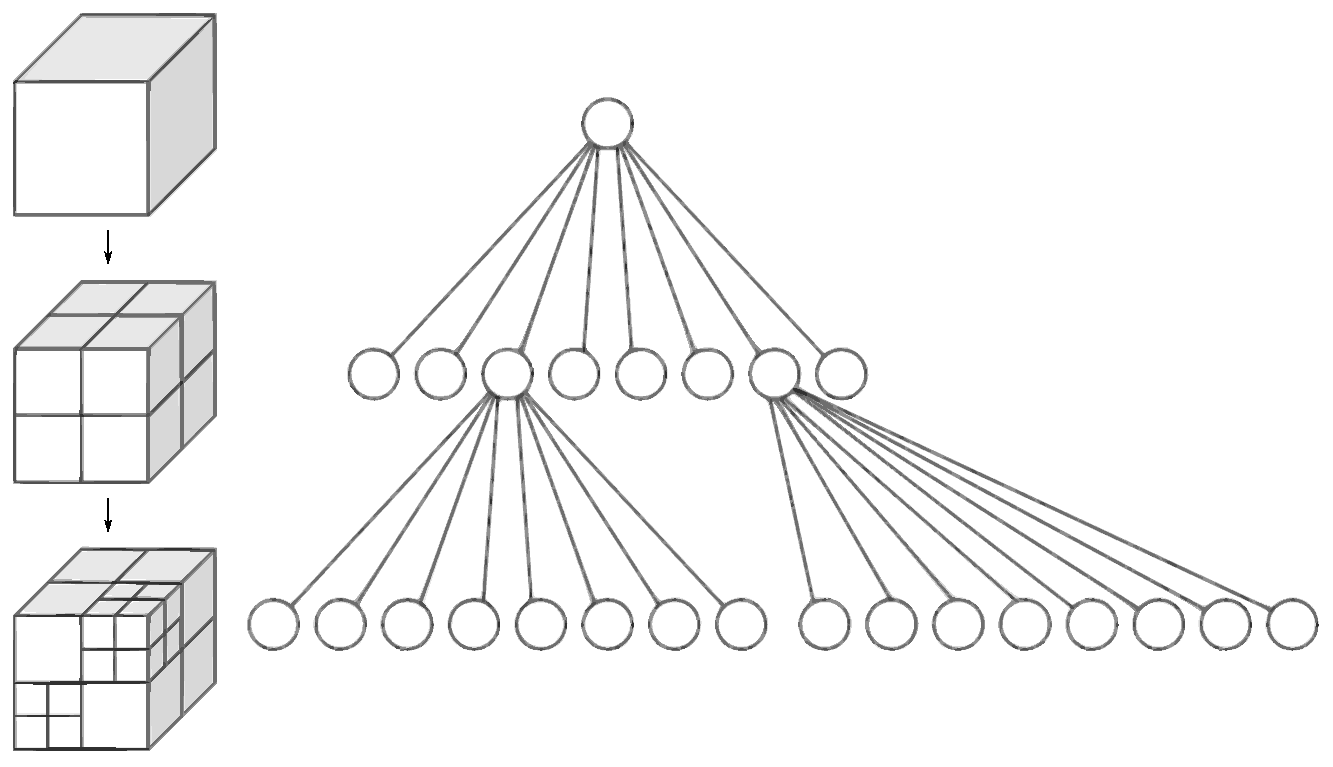
\includegraphics[scale=0.5]{images/octree.pdf}
 % octree.pdf: 640x368 pixel, 72dpi, 22.58x12.98 cm, bb=0 0 640 368
  \caption{Ein Octree der Tiefe 2. \textit{links: die räumliche Darstellung, rechts: die Baumdarstellung.}}
 \label{fig:basics:octree}
\end{figure}
In dieser Arbeit wurde jedoch eine spezielle Form des Octrees verwendet: der Loose Octree. Dieser erweitert den Octree um eine weitere Box pro Knoten: die sogenannte Loosebox. Sie teilt sich ihr Zentrum mit der Octree-Boundingbox, besitzt aber doppelte Kantenlängen. Wird nun festgestellt, dass in einem Knoten mehr als 5.000 Dreiecke liegen, wird die größe der einzelnen Dreiecke anhand der Loosebox geprüft. Liegt ein Dreieck vollständig in der Loosebox mit seinem Zentrum in der eigentlichen Boundingbox des Knotens, kann es weiter nach unten gereicht werden. Ist dies nicht der Fall, ist das Dreieck zu groß für den aktuellen Knoten und wird an den Vaterknoten gegeben (Abbildung \ref{fig:basics:looseoctree}).\\
Dies hat den Vorteil, dass große Dreiecke relativ weit oben im Baum zu liegen kommen und Kleinere entsprechend tief. Je größer ein Dreieck ist, desto größer ist auch die Wahrscheinlichkeit, dass das Dreieck sichtbar ist und somit gezeichnet werden muss. Bewegt man sich durch ein Modell, ist der Wurzelknoten, oder Szenen-Boundingbox, praktisch immer sichtbar, was bedeutet, dass die zur Wurzel gehörige Geometrie gezeichnet werden muss.
\begin{figure}
 \centering
  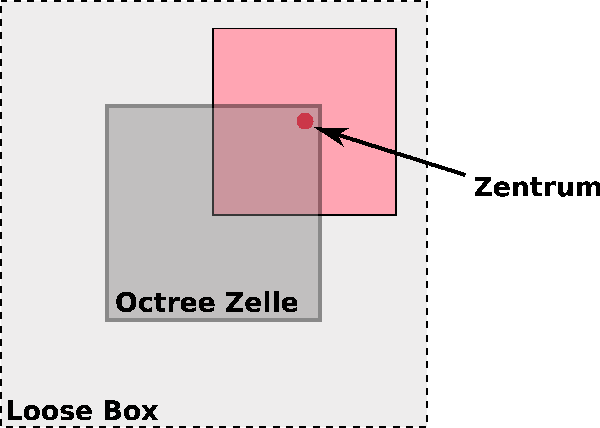
\includegraphics[scale=0.8]{images/looseoctree2.pdf}
  \caption{Ein Loose Octree in einer 2D-Darstellung. \textit{Das Zentrum des Objekts (rosa) befindet sich innerhalb der Octree Zelle, das gesamte Objekt befindet sich innerhalb der Loose Box.}}
 \label{fig:basics:looseoctree}
\end{figure}

\subsection{Randomized Sampletree}
\label{sec:basics:sampletree}
\todo[size=\small, inline, color=magenta]{Unterkapitel: Randomized Sampletree}
Als spezielle Ausprägung eines Loose Octrees gibt es den Randomized Sampletree \cite{klein}. Dieser unterschiedet sich von einem Octree darin, dass einzelne Dreiecke aus den tieferen Knoten nach oben gezogen wurden. Beim rendern der Szene wird in jedem Frame der Baum traversiert, um ein Frustum-Culling durchzuführen (siehe auch \ref{sec:basics:algos:frustumculling}). Ab einer bestimmten Tiefe im Baum wird die Traversion abgebrochen, um die Komplexität der Darstellung zu reduzieren. Dadurch kommt es allerdings zu Darstellungsfehlern, da nicht alle sichtbare Geometrie gerendert wird. An dieser Stelle schafft ein Randomized Sampletree abhilfe. Dadurch dass zufällige kleinere Dreiecke in höherliegenden Knoten gespeichert sind, werden diese auch gerendert. Ist die Flächensumme alle Dreiecke in einem Knoten des Sampletrees nicht größer als ein Pixel, wird die Traversion abgebrochen. Klein, Krokowski, Fischer et al. \cite{klein} haben gezeigt, dass diese Geometrie-Approximation von weit entfernten Objekten durch zufällige Dreiecke eine hinreichend korrekte Darstellung liefert. Dieses Verfahren wurde für komplexe geometrische Umgebungen entwickelt, weshalb es in dieser Arbeit verwendet wurde.
\begin{figure}
 \centering
  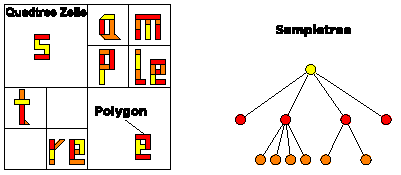
\includegraphics[scale=1.7]{images/sampletree2.pdf}
  \caption{Ein Sampletree in einer 2D-Darstellung. \textit{links: Eine Aufteilung von Polygonen in verschiedene Quadtree Zellen. rechts: Die Baumdarstellung des Sampletrees. Die farbigen Knoten geben an welche Polygonteile der linken Seite in welchen Knoten gespeichert wurden.}}
 \label{fig:basics:sampletree}
\end{figure}

\section{Computergrafik}
\label{sec:basics:computergrafik}
\todo[size=\small, inline, color=yellow]{Computergrafik $\rightarrow$ Spellcheck!}
Da Arbeitsspeicher in der Regel größer ist als der Speicher einer Grafikkarte, werden nicht alle geometrischen Objeke auf der Grafikkarte belassen. Wenn angeforderte Objekte bei einem Renderer eintreffen, werden die zunächst gar nicht an die Grafikkarte geschickt. Erst nach weiteren Tests, ob das Objekt immer noch sichtbar ist, findet der transfer zur GPU statt. Dort verbleiben sie dann, bis sie irgendwann aus platz- oder sichbarkeitsgründen verdrängt werden (siehe auch \ref{sec:basics:caching}). Um dies möglichst effizient umsetzen zu können werden Vertexbuffer Objects  (VBOs) genutzt. Die Idee ist dabei, dass Modelldaten, bestehend aus Vertices und Vertex-Normalen, in einem zusammenhängenden Speicherblock abgelegt werden. Ein Vertex besteht aus einer $xyz$-Koordinate und einer Vertex-Normalen. Der Zugriff auf Dreiecke erfolgt dann mittels einer Index-Liste, bei der immer drei Indices ein Dreieck ergeben. Alle Dreiecke eines Octree-Knotens wurden zu einem Vertexbuffer-Objekt zusammen gefasst (siehe \ref{sec:basics:octree}), da Geometrie innerhalb eines Knotens nicht weiter unterteilt wird. In Form von VBOs kann recht einfach entsprechender Platz im Grafik-RAM reserviert und die Daten in den Speicher geladen werden.\\
Im Gegensatz dazu verbleiben bei Vertex-Arrays alle Daten im Arbeitsspeicher des Rechners und werden für jeden Zeichenaufruf zur Grafikkarte übertragen. Vertex-Arrays bieten sich an, wenn Objekte nur einmal gezeichnet und dann verworfen werden. Von daher kommen sie nur auf den Datenknoten (siehe \ref{sec:impl:netzwerkarchitektur}) zum Einsatz, da diese ein getestetes Objekt nur in ihren Tiefenbuffer rendern und dann wieder verwerfen. Bei VBOs wäre der Overhead der Datenübertragung und der anschließenden Deallokation zu groß für eine einmalige Verwendung.

Das Modell der Boeing 777 besitzt auch Farbinformationen. Da bei CAD-Modellen Farben oft einen Hinweis auf den Produktionsort geben, ist die Anzahl der Farben beschränkt. Natürlich könnte man jedem Vertex eine Farbe zuordnen. Dies hätte jedoch zur Folge dass bei jedem Vertex die Farbe neu gesetzt werden muss, unabhängig davon, ob diese Farbe bereits gesetzt ist. Das würde jedesmal die Grafik-Pipeline unterbrechen und es wäre mit Geschwindigkeitseinbußen zu rechen. Deshalb wurden die Farben der Boeing, 32 an der Zahl, in einer 1D-Textur kodiert und die Texturkoordinate wurde als vierte Komponente an den Vertex gehängt. Wird nun ein Vertex gezeichnet, ersetzt der Vertex-Shader die harmonische vierte Komponente eines Vertices wieder durch $1.0$ und gibt die Textur-Koordinate an den Fragment-Shader weiter. Letzterer muss ohnehin eine Farbe schreiben, weshalb diese kurzerhand aus der Textur ausgelesen wird. Da die Anzahl der Farben bekannt ist ist, ergibt sich zur Berechnung der Texturkorrdinate der $i$-ten Farbe $\frac{i}{n}-\frac{1}{2n}$, wobei $n=$  Anzahl der Farben ist (Abbildung \ref{fig:basics:1dtexture}). Die Subtraktion der Hälfte eines Texels $\frac{1}{2n}$ ist Notwendig, da man sonst genau auf der Kante zwischen zwei Farben landet, was zu undefiniertem Farbverhalten in der Grafikkarte führt.
\begin{figure}
  \centering
  %%%%%%%%%%%%%%%%%%%%%%%%%%%%%%%%%%%%%%%%%%%%%%%%%%%%%%%%%
% 1D-Farbtextur mit Beschreibung und Labels
%%%%%%%%%%%%%%%%%%%%%%%%%%%%%%%%%%%%%%%%%%%%%%%%%%%%%%%%%


\begin{tikzpicture}
  \tikzset{ 
    every pin/.style={fill=yellow!50!white,rectangle,rounded corners=3pt,font=\small}, 
    small dot/.style={fill=black,circle,scale=0.3} } 
  \begin{axis}[
    x=13cm, y=1.0cm, 
    clip=false,
    ytick=\empty,
    xtick={0,0.03125,0.0625,0.09375,0.125,0.15625,0.1875,0.21875,0.25,0.28125,0.3125,
      0.34375,0.375,0.40625,0.4375,0.46875,0.5,0.53125,0.5625,0.59375,0.625,
      0.65625,0.6875,0.71875,0.75,0.78125,0.8125,0.84375,0.875,0.90625,0.9375,
      0.96875,1},
    xticklabels={$0$,$\frac{1}{n}$,$\frac{2}{n}$,$\frac{3}{n}$,$\frac{4}{n}$,$\frac{5}{n}$,$\frac{6}{n}$,$\frac{7}{n}$,$\frac{8}{n}$,$\frac{9}{n}$,$\frac{10}{n}$,
      $\frac{11}{n}$,$\frac{12}{n}$,$\frac{13}{n}$,$\frac{14}{n}$,$\frac{15}{n}$,$\frac{16}{n}$,$\frac{17}{n}$,$\frac{18}{n}$,$\frac{19}{n}$,$\frac{20}{n}$,
      $\frac{21}{n}$,$\frac{22}{n}$,$\frac{23}{n}$,$\frac{24}{n}$,$\frac{25}{n}$,$\frac{26}{n}$,$\frac{27}{n}$,$\frac{28}{n}$,$\frac{29}{n}$,$\frac{30}{n}$,
      $\frac{31}{n}$,$\frac{32}{n}$},
       %tickpos=right,
    major tick length={0.07cm},
    xtick align=outside,
    xtick pos=left,
    tick style={very thin, black},
    tick label style={
    font=\tiny},
    %major x tick num=5,
    %hide y axis,
    enlargelimits=false,
    axis on top] 
    \addplot graphics [xmin=0,xmax=1,ymin=0,ymax=1, 
      % trim=left bottom right top 
      includegraphics={trim=0 9 0 8,clip}
      ] 
      {images/colors.pdf}; 

\node[small dot,pin=-90:{$\frac{1}{2n}$}] at (axis description cs:0.017625,0) {}; 
%\node[small dot,pin=-45:{$\frac{1}{n}$}] at (axis description cs: 0.03325,0) {}; 

  \end{axis} 
\end{tikzpicture}

  \caption{1D-Farbtextur. $n=$Anzahl Farben. Um mittig auf den Texel der Farbe $i$ zuzugreifen, errechnet sich die Texturkoordinate durch $\frac{i}{n}-\frac{1}{2n}$. }
  \label{fig:basics:1dtexture}
\end{figure}

\section{Approximation}
\label{sec:basics:approximation}
\todo[size=\small, inline, color=blue!40]{Kapitel: Approximation}
Approximationen in der Computergrafik haben oft  Zurfolge, dass die Bildqualität verringert wird. Sei es weil Objekte in niedrigeren Auflösungen
\begin{itemize}
 \item Teile können weggelassen werden
 \item Tiefenbuffer Update nur alle paar Frames
\end{itemize}

\section{Algorithmen}
\label{sec:basics:algos}
\todo[size=\small, inline, color=blue!40]{Kapitel: Algorithmen}
\begin{itemize}
  \item Occlusion Culling \cite{RTR3}\label{sec:basics:algos:occlusionculling}
  \item Frustum Culling \cite{RTR3} \label{sec:basics:algos:frustumculling}
  \item c-Collision Protokoll zur Lastbalancierung im Netzwerk \label{sec:basics:algos:ccollision} \ref{chap:relwork}
  \item c-Collision?: \cite{DBLP:conf/arcs/RehbergS99}: \textit{Almost optimal schedules with a simple protocol}
  \item \underline{adpative collision / c-Load}, gewichtet: \cite{ccol2}: \textit{Allocating weighted jobs in parallel}
  \begin{itemize}
    \item Untere Schranke in Abhängigkeit von Runden \& Körben => keine Bälle
    \item Obere Schranke Durchschnittsgewicht + maximales Gewicht
    \item w.h.p. = with high probability
    \item i.u.r. = independendly and uniformly at random
    \item c-Load Collision Protocol:
    \begin{itemize}
      \item wähle parallel für jeden Ball zufällig 3 Körbe
      \item Jeder Ball schickt an diese 3 Körbe einen Request samt Gewicht
      \item Jeder Korb berechnet die Summe alle Gewichte der requests an ihn. Ist die Summe höchstens c -> akzeptiere, sonst lehne ab.
      \item Bekommt ein Ball mindestens ein Accept, lösche den Ball.
    \end{itemize}
    \item Adaptive Collision Protocol:
    \begin{itemize}
      \item wähle parallel für jeden Ball zufällig 3 Körbe
      \item Jeder Ball schickt an diese 3 Körbe einen Request samt Gewicht
      \item Jeder Korb berechnet die Summe alle Gewichte der requests an ihn. Ist die Summe höchstens c -> akzeptiere, sonst lehne ab.
      \item Bekommt ein Ball mindestens ein Accept, lösche den Ball.
    \end{itemize}
    \item Conclusion:
    \begin{itemize}
      \item Untere Schranke für $m \ge n$ Bälle in $n$ Körbe.
      \item ein dritter Korb ist nicht notwendig.
    \end{itemize}


  \end{itemize}
  \item c-Collision Basics: \cite{ccol3}: \textit{Parallel Balanced Allocations}
  \begin{itemize}
    \item $m$ Bälle in $n$ Körbe
  \end{itemize}
  \todo[size=\small, inline]{c-Collisionprotokoll-Erklärung!}%
  \begin{itemize}
    \item auch bälle in Körbe aber diesmal haben die Bälle Gewichte
  \end{itemize}

\end{itemize}

\subsection{Caching}
\label{sec:basics:caching}
\todo[size=\small, inline, color=blue!40]{Kapitel: Caching}
\begin{itemize}
 \item wird über Algos gefüllt
\end{itemize}

\subsection{Speichermanagement}
\label{sec:basics:speichermanagement}
\todo[size=\small, inline, color=blue!40]{Kapitel: Speichermanagement}
\begin{itemize}
 \item nicht jeder braucht alles -> Kacheln
 \item Gewichtung über die Anzahl der Dreiecke pro Request
\end{itemize}
